\section{Log Extension} \label{sec:log}
If we allow small, but significant, changes to the CT landscape, it is possible
to avoid inclusion verification and the involved complexities as described in
Section~\ref{sec:auditor}.  The idea is based on returning back to the premise
of some, but not all, CT logs being honest.  However, the goal is not only
\emph{resilience towards} but also \emph{detection of} CT logs that misbehaved.
The extended design idea is shown in Figure~\ref{fig:ext-log}.  Tor
Browser submits presented SFOs probabilistically to CTRs that are selected
at random, and CTRs store the submitted SFOs before any auditing takes place.
Here, auditing refers to adding an SFO to an independent CT log; not just the
underlying certificate chain.  By also adding the issued SCTs, the associated CT
logs can be held accountable for possible omissions.

\begin{figure*}
    \centering
    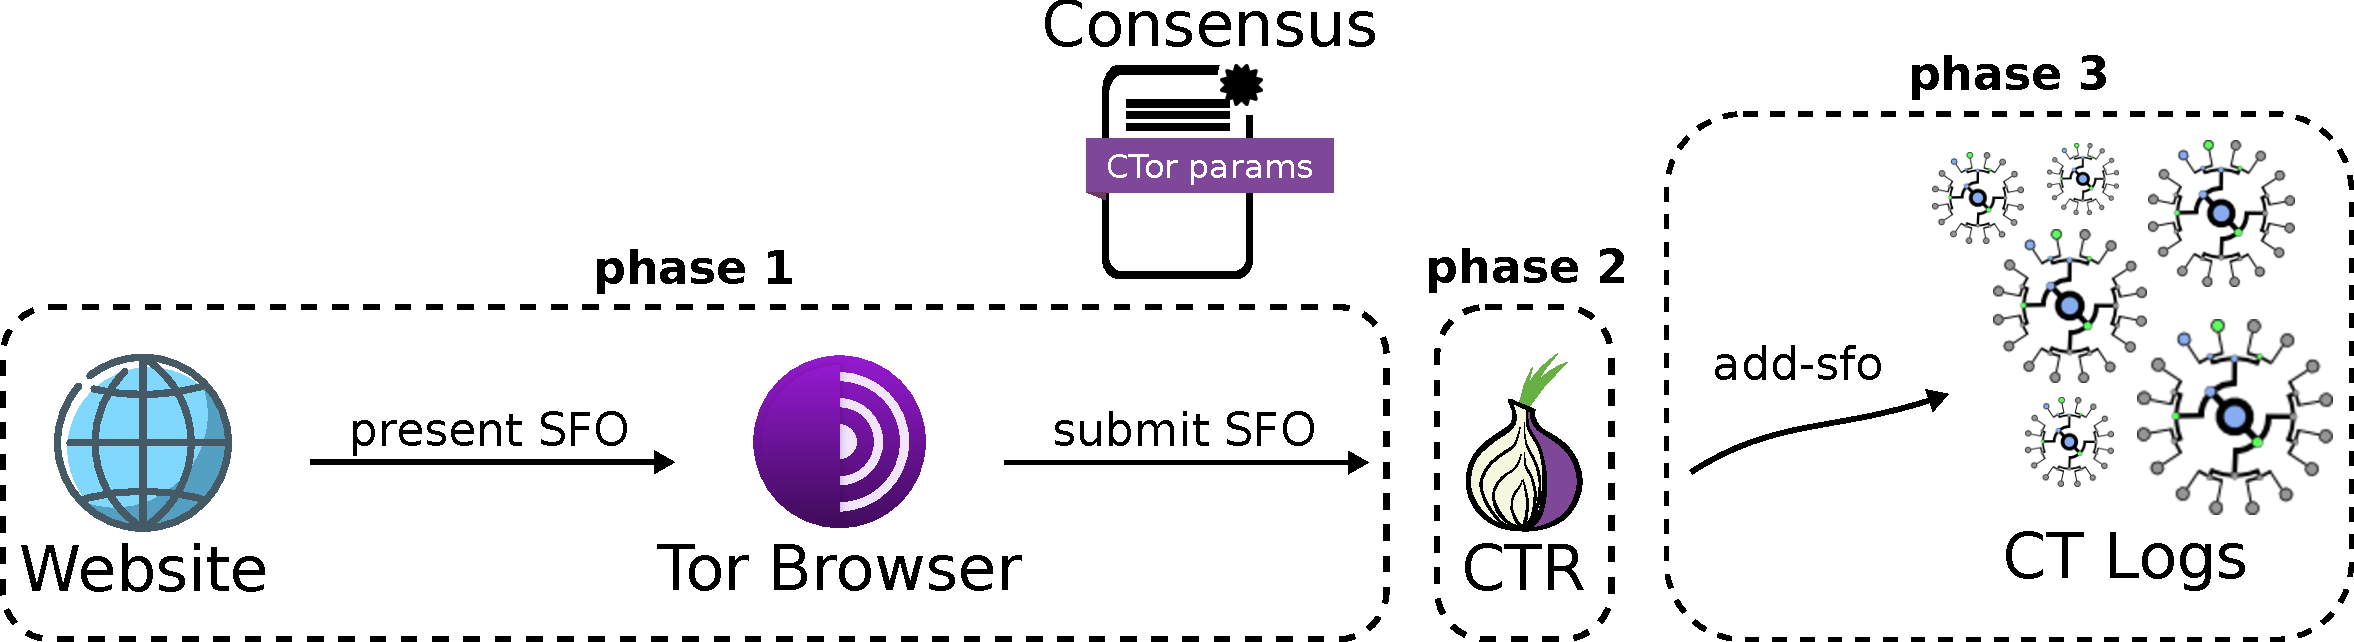
\includegraphics[width=0.85\textwidth]{img/design-log}
	\caption{The updated design of CTor to capture cryptographic evidence of CT
	log omission. The key difference to the previous design (shown in
	Figure~\ref{fig:design-ca}) is the new API call used at CT logs.}
    \label{fig:ext-log}
\end{figure*}

The prerequisite for such an extension to work is that CT logs support an
additional endpoint:
	\texttt{add-sfo}.
First we describe how this endpoint could be operated so that \emph{the only
change} with regards to the base design in Section~\ref{sec:base} is that
certificate chains and SCTs are added.  Next, we explain how some of the log's
complexity could be moved into the Tor landscape at the cost bringing back the
threat of flooding as discussed in Section~\ref{sec:auditor:analysis:phase2}.

\textbf{Approach~1.}
Recall from Section~\ref{sec:auditor:design:phase2} that there must not be any
early signals that allow misbehaving CT logs to reactively merge certificate
chains before any MMD promise is violated.  To ensure that this is the case, the
\texttt{add-sfo} endpoint could entail a promise that the added SFO will not be
merged until all MMDs elapsed.\footnote{%
	Two options: just base on MMD and wait ``long enough'', or wait until the
	log created an actual STH.  TODO: refactor me.
} For example, the SCT that is returned by the \texttt{add-sfo} endpoint could
have a future-dated timestamp without violating any policy aspect of
CT/bis~\cite{ct/bis}.  Note that the appeal of letting CT logs handle
\emph{delayed merges} is that no attacker within Tor's threat model have high
certainty of succeeding with a network-wide flush.

\textbf{Approach~2.}  The other option is to suggest minimal changes to the CT
landscape by operating the \texttt{add-sfo} endpoint without any other
expectation than that it must allow SCTs in addition to a certificate chain.
To avoid early signals, CTRs should adopt the procedures in
Sections~\ref{sec:auditor:design:phase2}--\ref{sec:auditor:design:phase3}
or something similar.  For example, \texttt{audit\_after} timestamps
could be computed conservatively as in Figure~\ref{fig:audit-after-cons}
to remove the dependency of STHs in the Tor consensus.  There is a threat of
network-wide flushes regardless, and the extra-info document should therefore be
extended as in Section~\ref{sec:auditor:extra-info}.

%
% TODO:
% Think we need either 2*MMD as the log must produce an STH every MMD.  Or,
% have STHs in the consensus after all which would be more robust.
%
\begin{figure}
	\centering
	TODO: discuss and docdoc.
	\caption{%
		Algorithm that computes a conservative \texttt{audit\_after} timestamp
		$t$.
	}
	\label{fig:audit-after-cons}
\end{figure}
